\documentclass[10pt,a4paper]{amsart}

\usepackage{graphicx}
\usepackage{caption}
\usepackage{subcaption}
\usepackage{sidecap}

\author{Vaibhav Karve\\Derrek Yager}
\title{Progress report on study of NYC traffic}

\begin{document}

\date{\today}
\maketitle

\section{Restricting to a block}
We restrict our attention to the block between W. 44th to 45th St. and
8th to 9th Ave. This block was selected at random. On extracting the
data from the data file for 2011, we see that these streets are all one-way
access only.

\subsection{Naming convention}
\subsubsection{Intersections}
	\begin{itemize}
		\item \(A=\) W. 44th St. and 8th Ave. (Node\_id = 42435671)
		\item \(B=\) W. 44th St. and 9th Ave. (Node\_id = 42443561)
		\item \(C=\) W. 45th St. and 8th Ave. (Node\_id = 42432700)
		\item \(D=\) W. 45th St. and 9th Ave. (Node\_id = 42432703)
	\end{itemize}

\subsubsection{Roads}
	\begin{itemize}
		\item \(BA\) (Link\_id = 128255)
		\item \(AC\) (Link\_id = 169017)
		\item \(CD\) (Link\_id = 182993)
		\item \(DB\) (Link\_id = 181188)
	\end{itemize}
		
We restrict our attention to only these links, one at a time. For each
link, from the database, we extract 2 separate arrays: one giving the
average travel time in seconds, for every hour of the year; and the other
giving the number of trips on that used that link, for every hour of the
year.


\subsection{Periodicity analysis}
\subsubsection{Stratifying the data}
Intuitively, one may expect that traffic patterns repeat themselves
every \(7\) days (weekly) or maybe every \(30\) days (monthly). Or
perhaps, there is no such periodicity. Whatever be the case, the
periodicity should not be imposed, but rather should be inferred
from the data itself. To do so, we we assume a particular period in
days, call it \texttt{period} and divide the entire data into
\(24\times\mathtt{period}\) number of bins. This converts our data
from flat lists of trips and traveltimes to something that may be
viewed as stratified data. 

Stratified data now looks like:

\[\bordermatrix{
	~ & \text{Cycle 1} & \text{Cycle 2} & \cdots &\text{Cycle }\left(
		\lfloor\frac{365}{\mathtt{period}}\rfloor+1\right)&\cr
	\qquad\text{Stratum 1} & 5 & 2 & \cdots & 10 \cr
	\qquad\text{Stratum 2} & ? & 7 & \cdots & 5 \cr
	\qquad\qquad\vdots & \vdots & \vdots & ~ & \vdots \cr
	\text{Stratum 24*\texttt{period}-1} & 33 & ? & \cdots & ? \cr
	\text{Stratum 24*\texttt{period}} & ? & 32 & \cdots & ? \cr	}\]

Here, number of rows \(=24\times\mathtt{period}\). We let period range from
\(2\) to \(38\) for our periodicity analysis. As an illustration, we show
below the special case when \(\mathtt{period} = 7\) i.e., cycles are weeks.

\[\bordermatrix{
	~ & \text{Week 1} & \text{Week 2} & \cdots & \text{Week 53} & \cr
    	\text{Sat 0000-0100 hrs} & 5 & 2 & \cdots & 10 \cr
    	\text{Sat 0100-0200 hrs} & ? & 7 & \cdots & 5 \cr
    	\qquad\qquad\vdots & \vdots & \vdots & ~ & \vdots \cr
	\text{Fri 2200-0300 hrs} & 33 & ? & \cdots & ? \cr
	\text{Fri 2300-0000 hrs} & ? & 32 & \cdots & ? \cr	}\]

Note that the trailing values in the last column will need to be set to (?)
because a year does not contain \(53\) full weeks and there will be data
points ``missing'' in the last week.

\subsubsection{Missing values}
The question marks (?) in the above matrix correspond to those hours for which
we have no data on our link. This ofcourse does not mean that there is no
traffic on that link at that time, just that we don't know what it it. These
are to be treated as missing values in our data and need to be somehow
inferred.

The links \(BA\), \(AC\), \(CD\) and \(DB\) have \(20\%\), \(0\%\), \(0\%\)
and \(1\%\) of their values missing, respectively.

The most natural first approximation for these missing values is the mean
value of the corresponding stratum to which each missing value belongs.

The Inferred Stratified data looks like:
\[\bordermatrix{
	~ & \text{Cycle 1} & \text{Cycle 2} & \cdots &\text{Cycle }\left(
		\lfloor\frac{365}{\mathtt{period}}\rfloor+1\right)&\cr
	\qquad\text{Stratum 1} & 5 & 2 & \cdots & 10 \cr
	\qquad\text{Stratum 2} & Mean_1 & 7 & \cdots & 5 \cr
	\qquad\qquad\vdots & \vdots & \vdots & ~ & \vdots \cr
	\text{Stratum 24*\texttt{period}-1} & 33 & Mean_2 & \cdots & Mean_n \cr
	\text{Stratum 24*\texttt{period}} & Mean_1 & 32 & \cdots & Mean_n \cr	}\]
where \(n=\left(\lfloor\frac{365}{\mathtt{period}}\rfloor+1\right)\). Here, we
calculated the mean for each stratum by ignoring the missing values.

\subsubsection{Stratified variances}
To establish the optimal choice of \texttt{period} for the data, we calculate
the variance of the inferred stratified data we obtained in the previous
subsection.
	\[\text{Variance of stratified data} \approx \frac{1}{n}
		\sum_n{\text{Variance of each stratum}}\]
where \(n=24\times\mathtt{period}\) is the total number of strata.

If there truly does exist a periodicity in the data, for the correct
\texttt{period}, the values within each stratum will lie close to each other
and hence, the variance will be minimized. Hence, we look for dips in the
variance.

\subsubsection{Conclusion of periodicity analysis}
We calculate the variance for each value of \texttt{period} from \(2\) to
\(38\). The graph of the variances for link \(BA\) for the No.\ of Trips
during 2011 is given below:

\begin{figure}[hbtp]
\centering
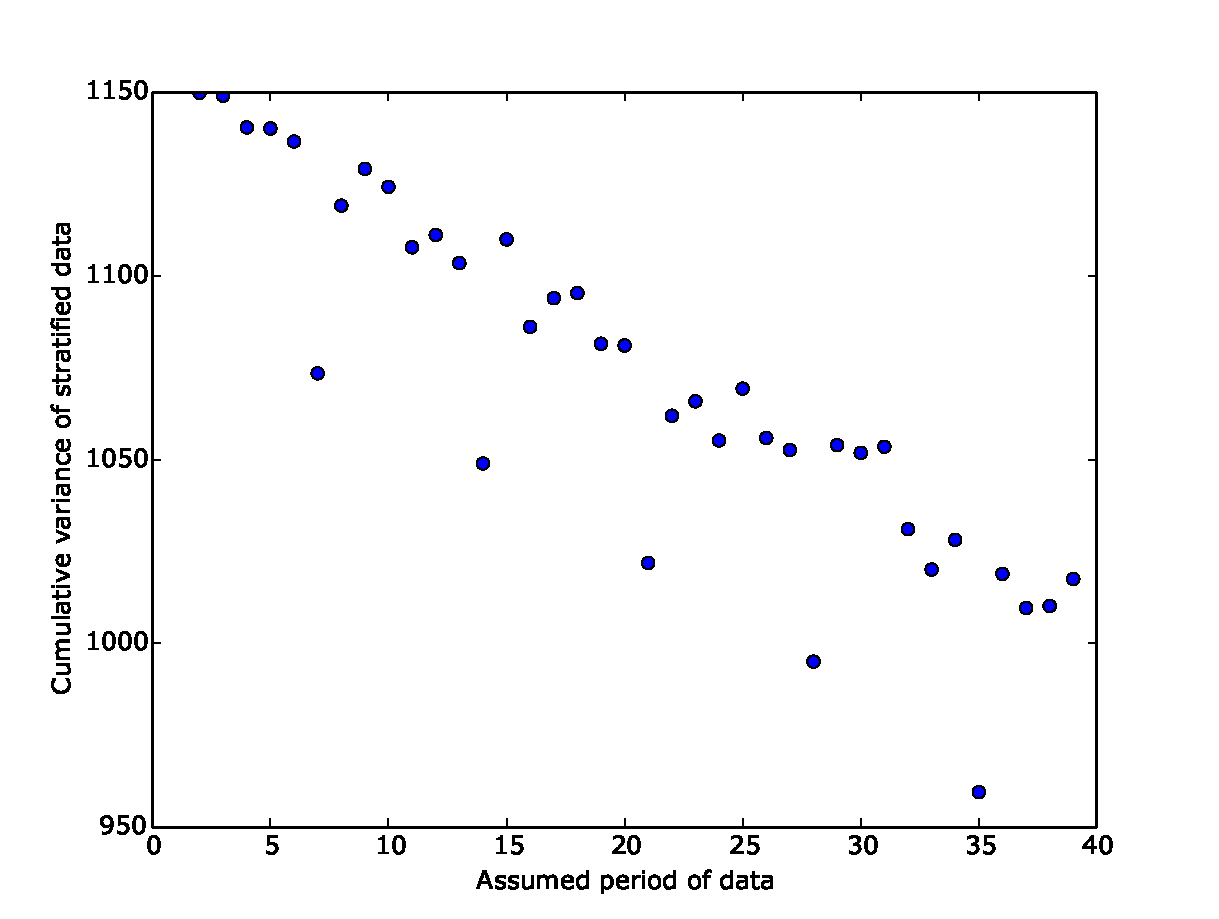
\includegraphics[scale=0.5]{Figures/Periodicity_analysis_BA_Trips.pdf} 
\caption{The dips in variance correspond to \(\mathtt{period}=7,14,21,35\).}
\end{figure}

The other three links show similar dips in variance at \texttt{period} values
which are multiples of \(7\), in both data -- Travel times as well as No.\ of
Trips. \textbf{Conclusion:} NYC traffic data has a \(7\)-day periodicity.

\subsection{Periodicity analysis via autocorrelation}
An easier, and more standard way to establish periodicity would be to
calculate the autocorrelation of our data for four links assuming different
lags (\texttt{period} values) of \(1\) to \(39\) days.

For a discrete set of observations \(\{X_1, X_2, \ldots, X_n\}\), an estimate
of the autocorrelation can be obtained as,
	\[\widehat{\mbox{Autocorrelation}}(k) = \frac{1}{(n-k)\sigma^2}
		\sum_{t=1}^{n-k}(X_t-\mu)(X_{t+k}-\mu)\]
where \(k=24\times\mathtt{period}\) is the lag in hours for which we are
testing autocorrelation in our data, and \(\mu\) and \(\sigma^2\) are the mean
and variance of the data respectively.

\subsubsection{Missing values}
We calculate the mean (\(\mu\)) of the data, ignoring the missing values. We
then replace the missing values with \(\mu\). We calculate the variance
(\(\sigma^2\)) of this \emph{corrected} data.
We then proceed to calculate the autocorrelation for different values of
\texttt{period} using the formula mentioned in the previos subsection.

\subsubsection{Conclusion of autocorrelation study}
We plot the autocorrelations for Trips data and Traveltimes seperately, for
all four road links simultaneously. The autocorrelation is high for
\texttt{period} values that are a multiple of \(7\). This confirms what was
seen by the statifying the data -- NYC traffic patterns repeat every seven
days.

\begin{figure}[h!]
\centering
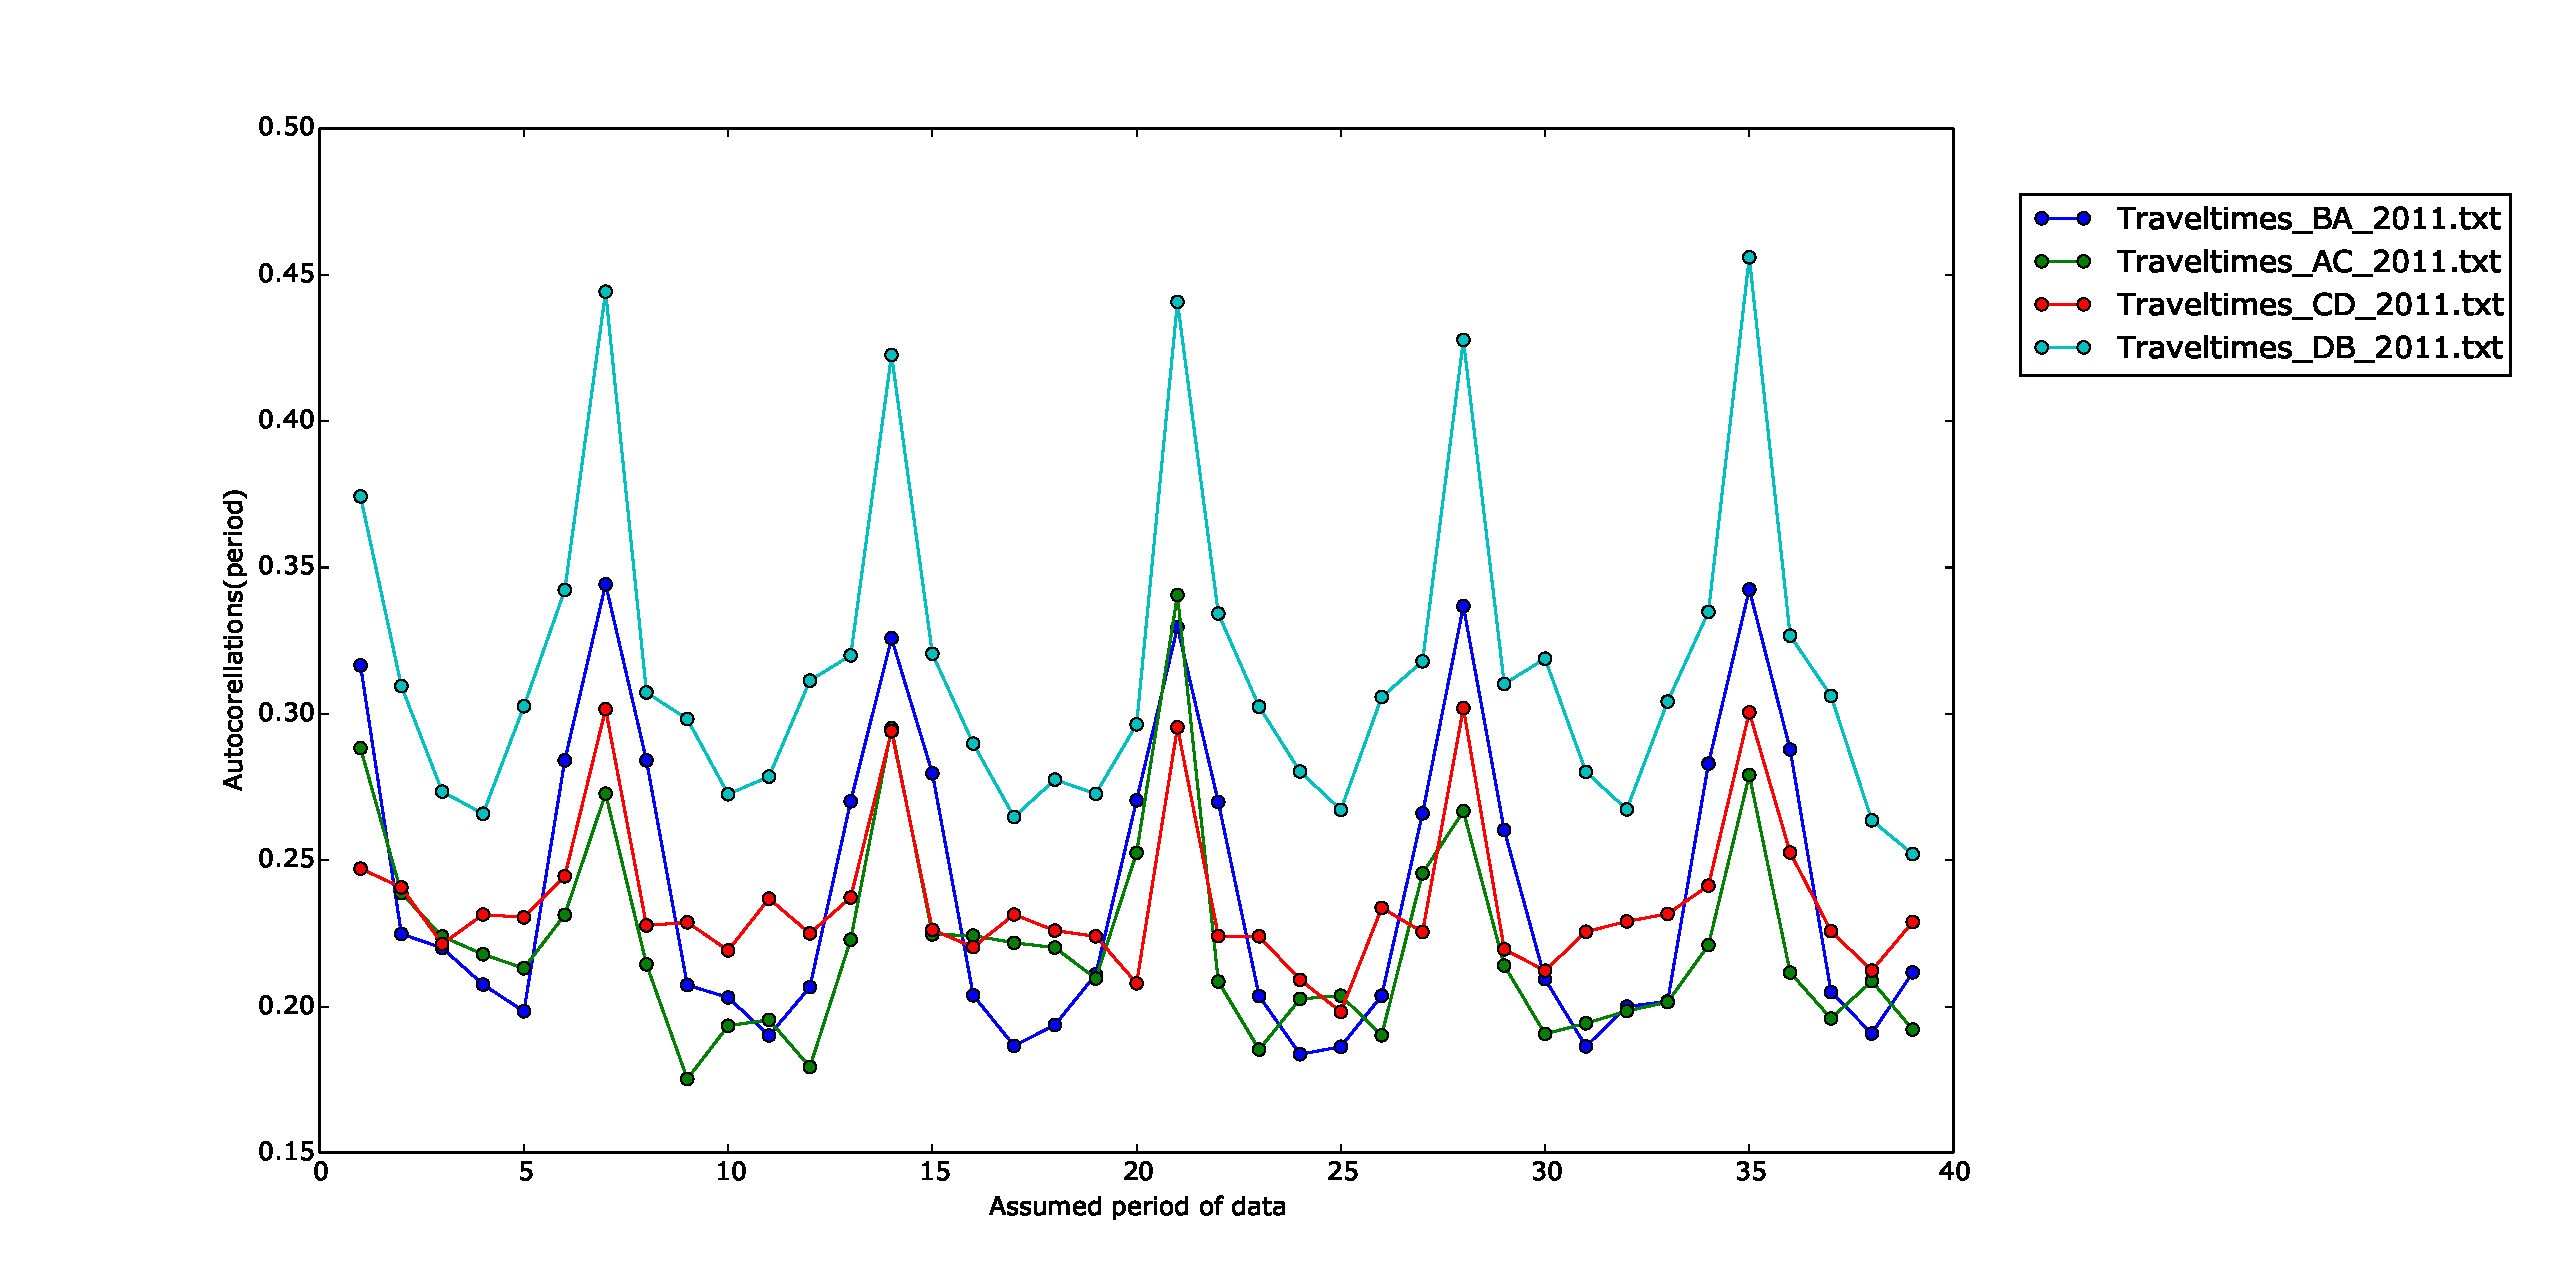
\includegraphics[scale=0.35]{Figures/Autocorrelation_Traveltimes.pdf}
\caption{Autocorrelations for Travel-times data of all four road links. The
peaks in
autocorrelation correspond to \(\mathtt{period}=7,14,21,35\).}
\end{figure}

\begin{figure}[h!]
\centering
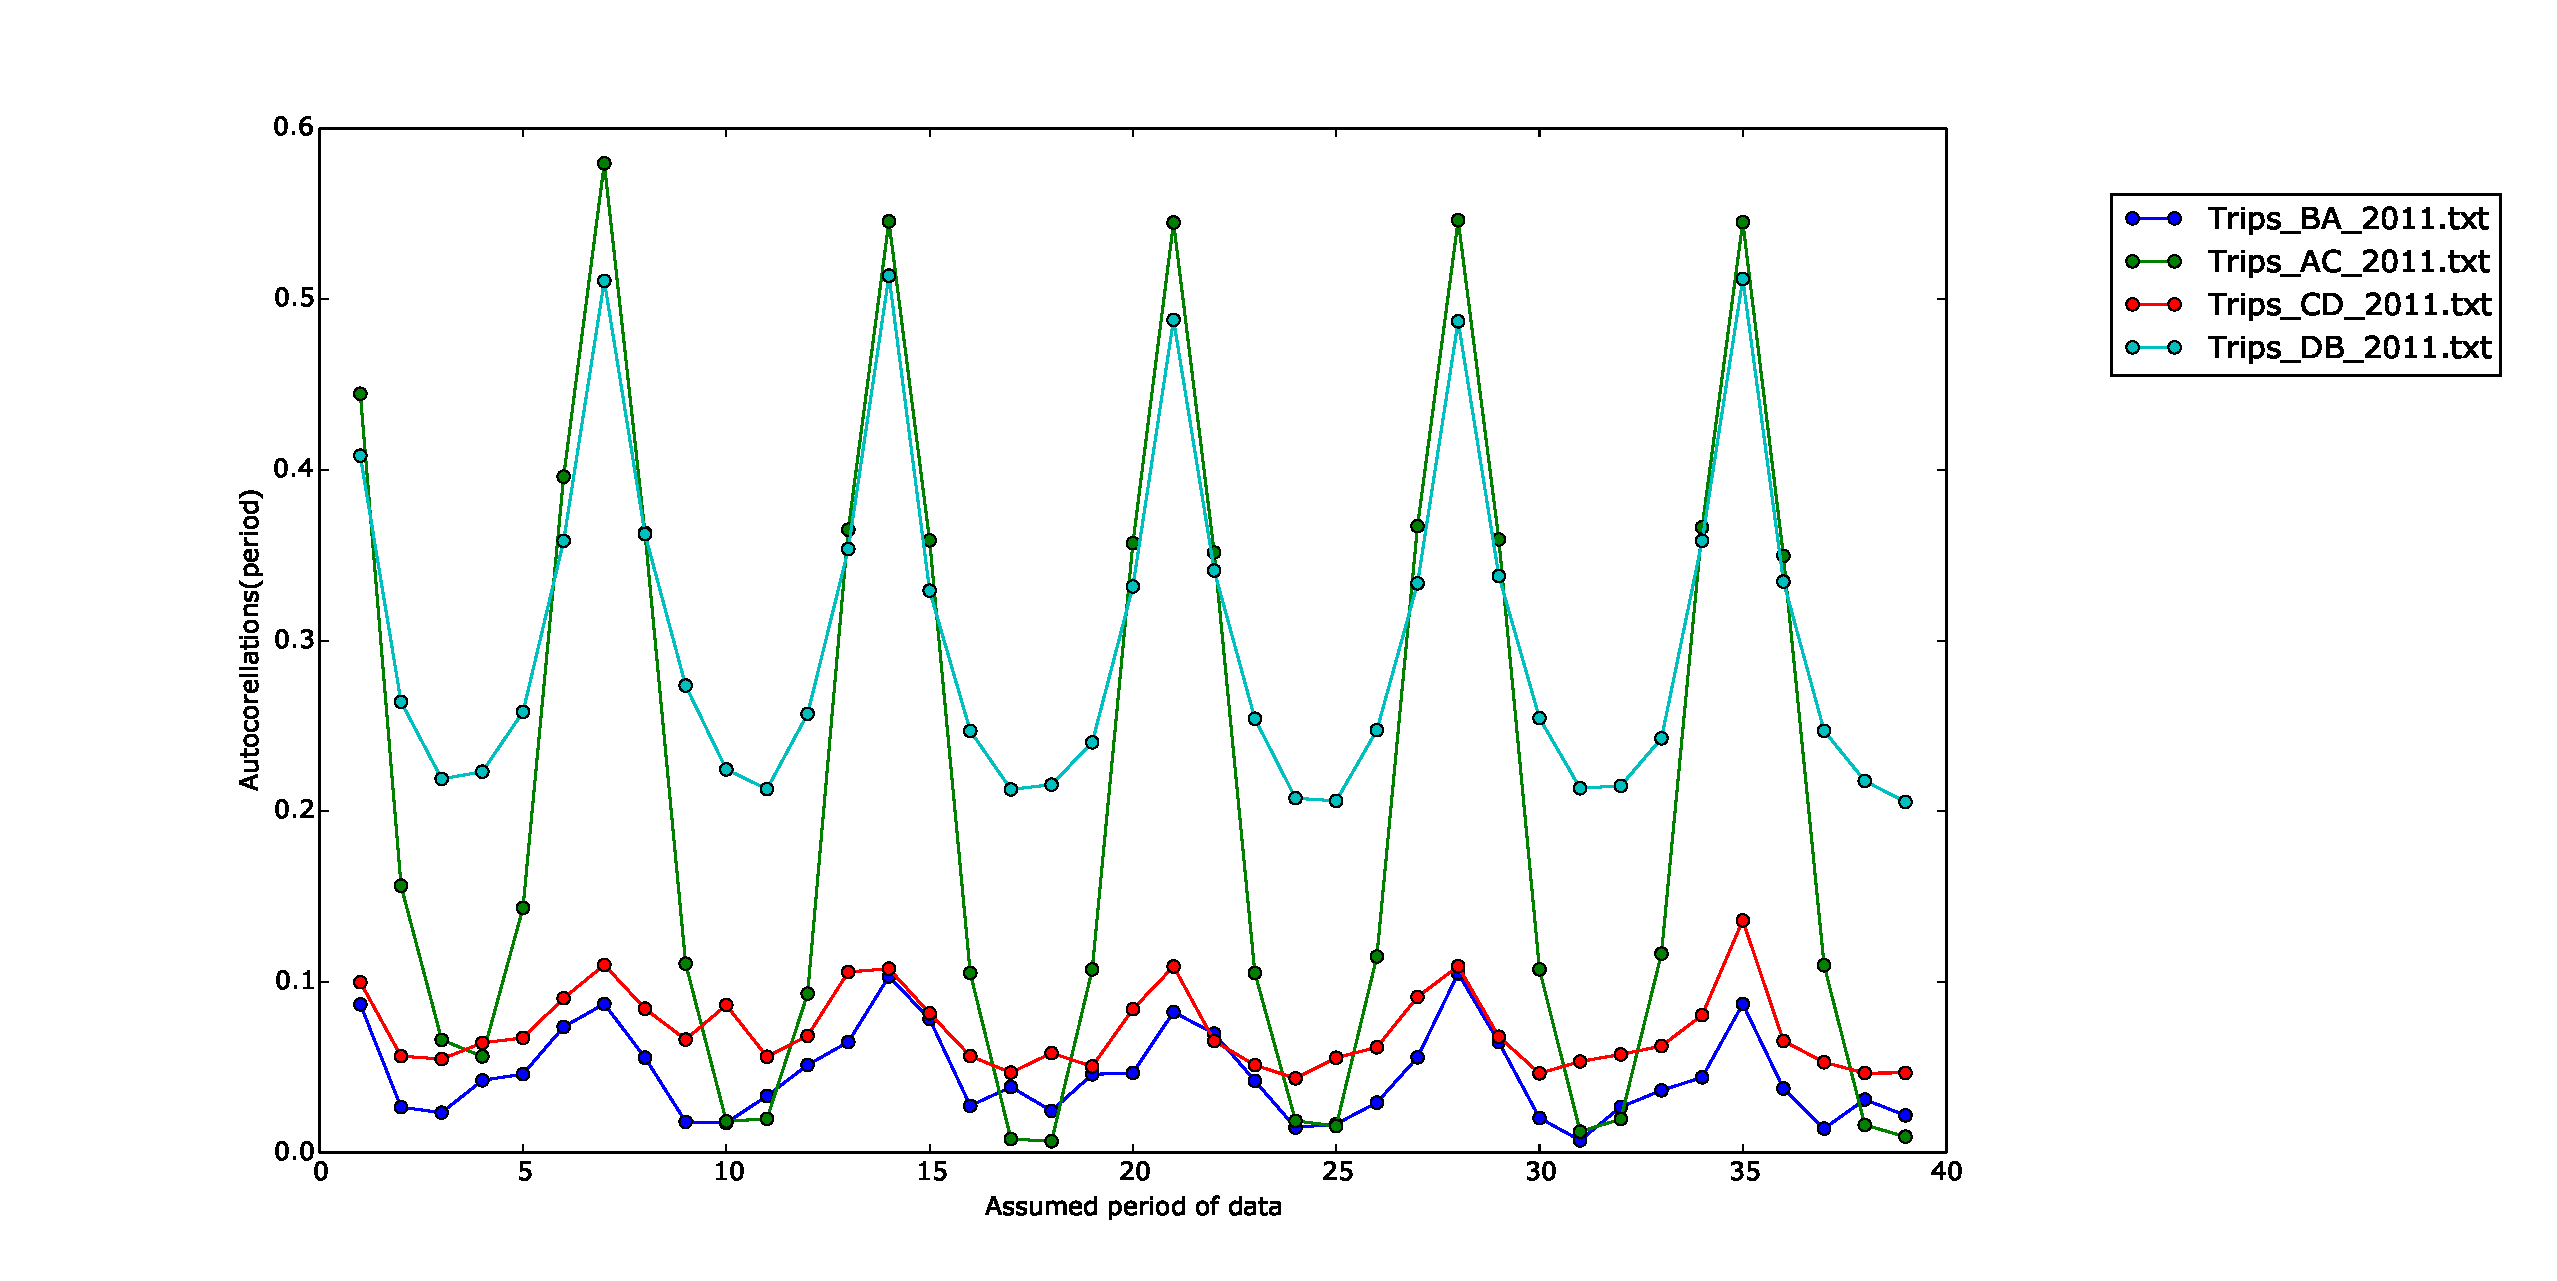
\includegraphics[scale=0.35]{Figures/Autocorrelation_Trips.pdf}
\caption{Autocorrelations for Trips data of all four road links. The peaks in
autocorrelation correspond to \(\mathtt{period}=7,14,21,35\).}
\end{figure}

\newpage
\subsection{Visualizing the data}
Keeping in view the conclusions drawn from the autocorrelation analysis,
henceforth, we try to analyze each dat of the week seperately. We try to
visualize the data by plotting different parts of the data file, in the hopes
that it will point towards directions in which we can carry out further study. 

\subsubsection{Daily pattern}
Below are shown the graphs for each day of the week. These plots are also
overlaid with the \(r=1\) results from Non-negative Matrix factorization. NMF
is discussed in greater detail in the next section.

\begin{figure}[h!]
    \begin{subfigure}[b]{0.5\textwidth}
        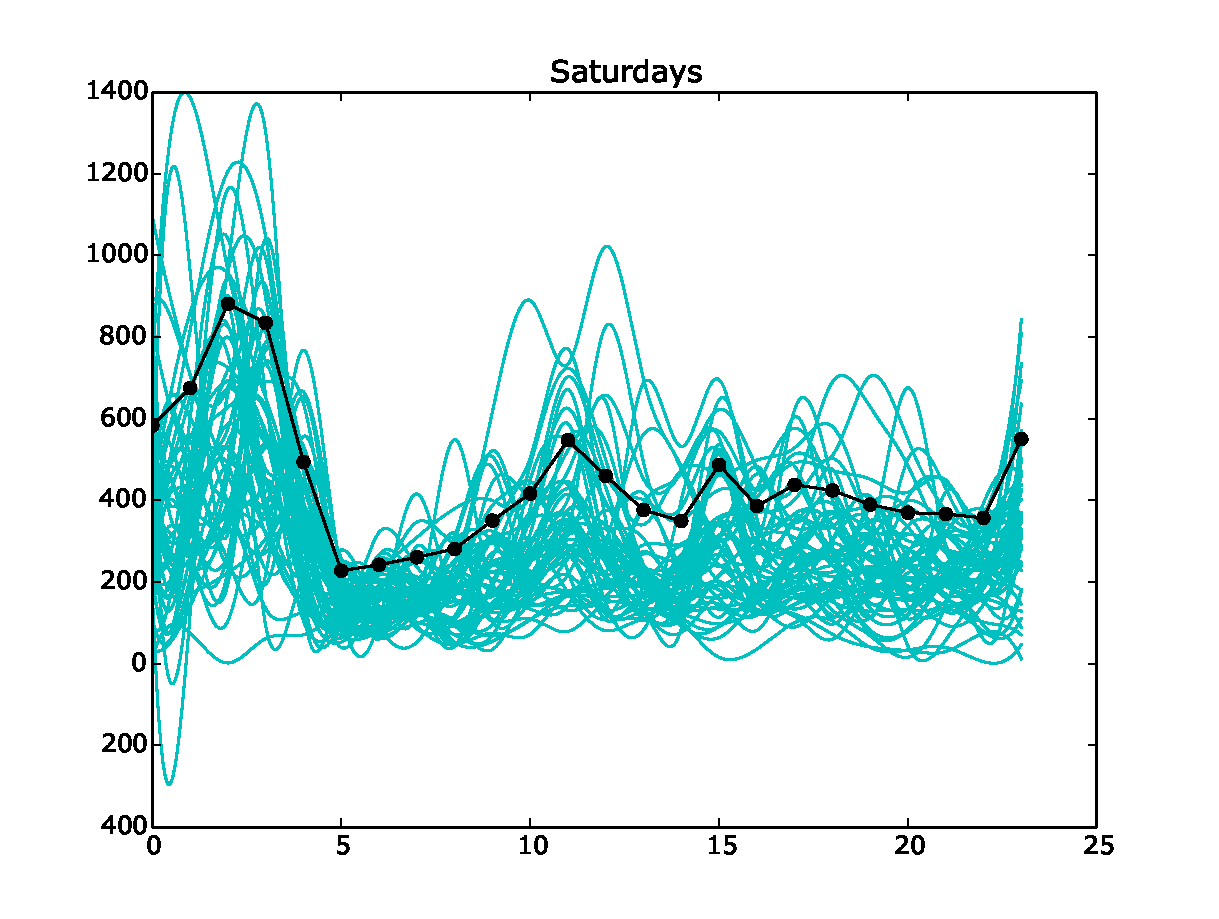
\includegraphics[width=\textwidth]
	        {Figures/Daily_trends_AC_Saturday.pdf}
    \end{subfigure}
    ~
    \begin{subfigure}[b]{0.5\textwidth}
        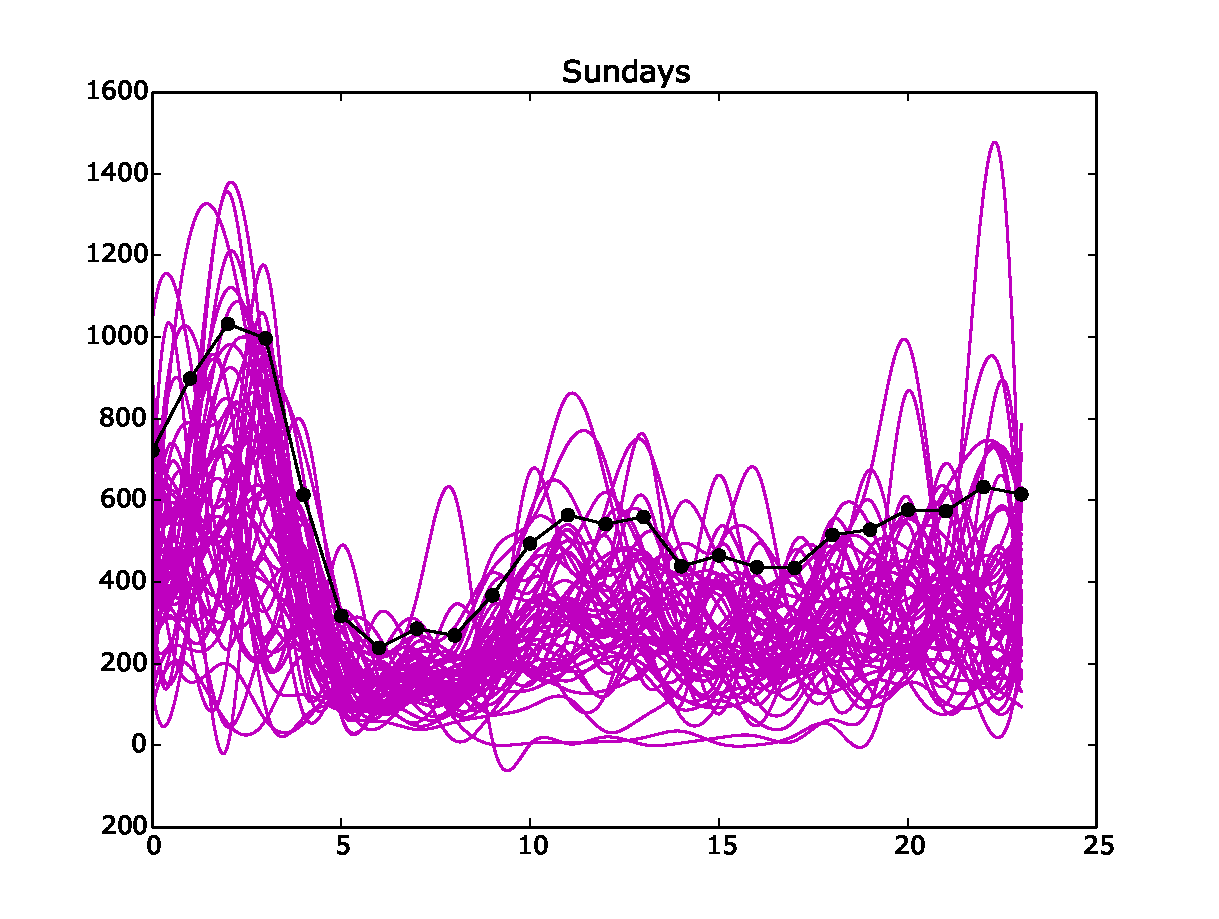
\includegraphics[width=\textwidth]
       		{Figures/Daily_trends_AC_Sunday.pdf}
    \end{subfigure}

    \begin{subfigure}[b]{0.5\textwidth}
        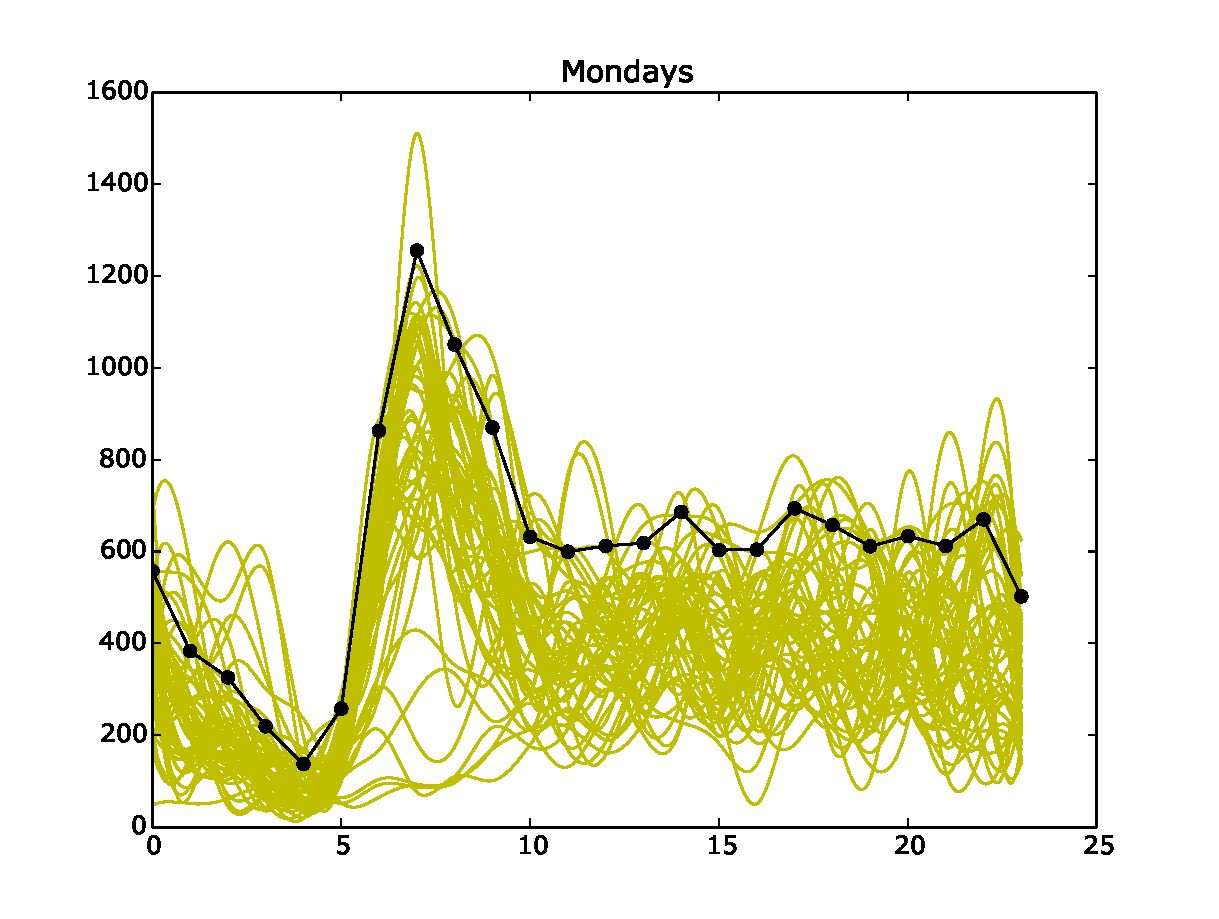
\includegraphics[width=\textwidth]
        		{Figures/Daily_trends_AC_Monday.pdf}
    \end{subfigure}
    ~
    \begin{subfigure}[b]{0.5\textwidth}
        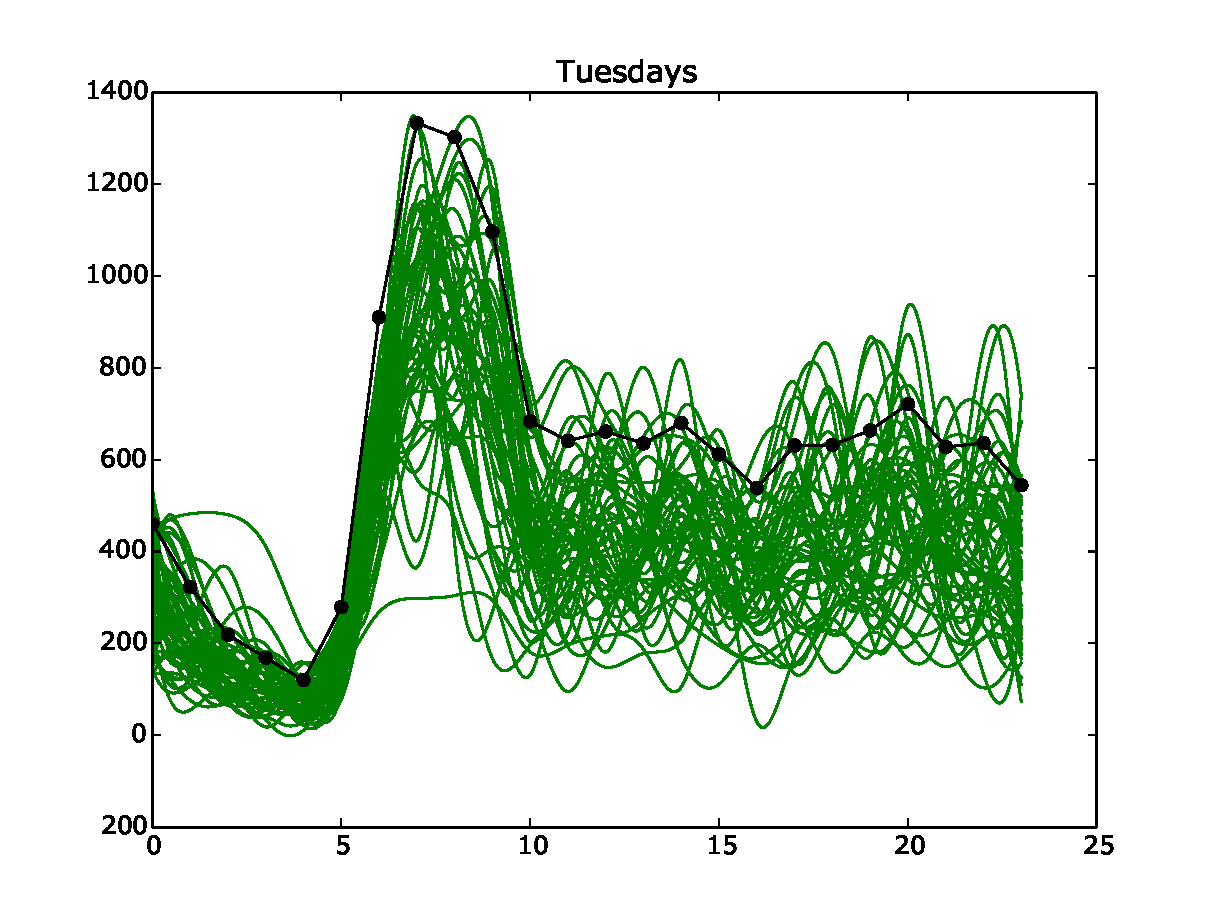
\includegraphics[width=\textwidth]
        		{Figures/Daily_trends_AC_Tuesday.pdf}
    \end{subfigure}

    \begin{subfigure}[b]{0.5\textwidth}
        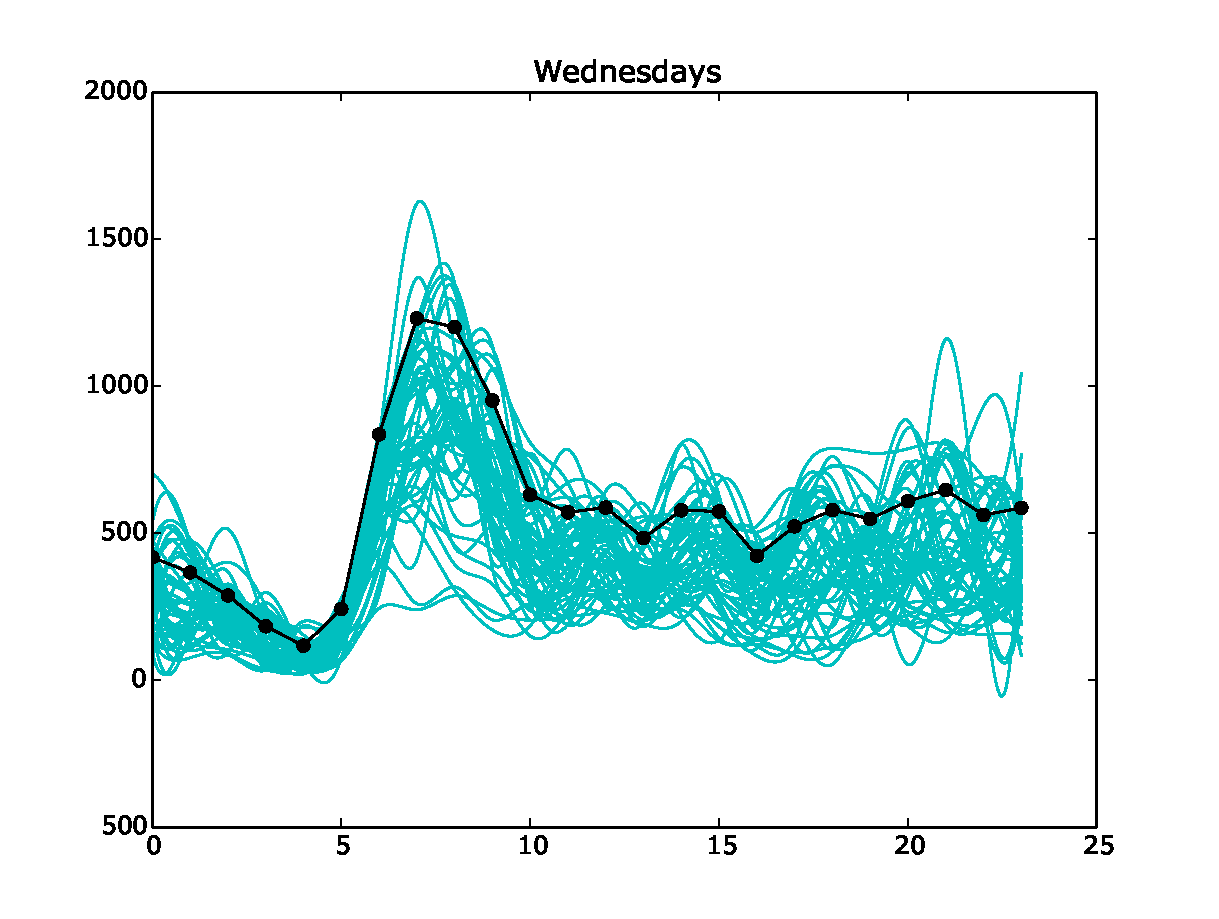
\includegraphics[width=\textwidth]
        		{Figures/Daily_trends_AC_Wednesday.pdf}
    \end{subfigure}
    ~
    \begin{subfigure}[b]{0.5\textwidth}
        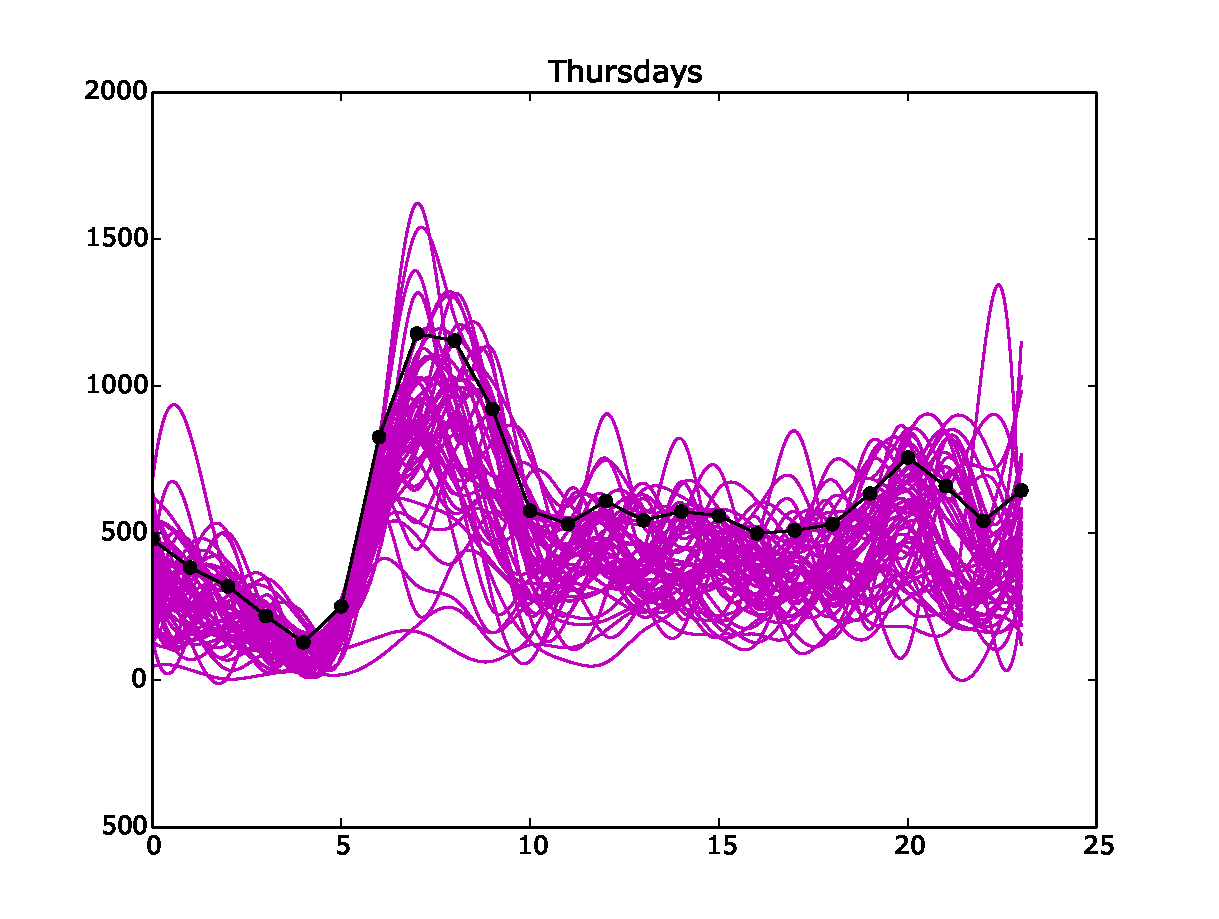
\includegraphics[width=\textwidth]
        		{Figures/Daily_trends_AC_Thursday.pdf}
    \end{subfigure}
    
    \begin{subfigure}[b]{0.5\textwidth}
        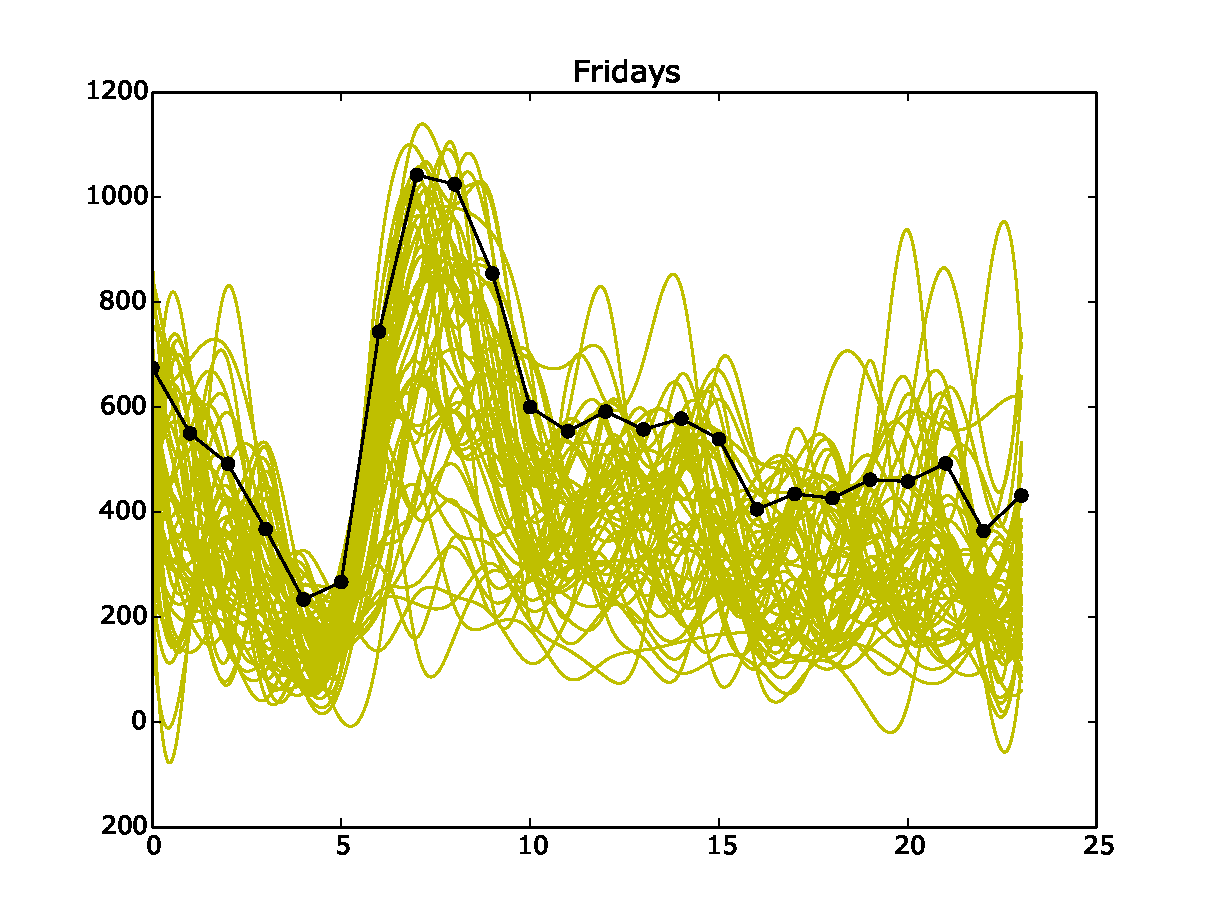
\includegraphics[width=\textwidth]
        		{Figures/Daily_trends_AC_Friday.pdf}
    \end{subfigure}
    ~
    \begin{subfigure}[b]{0.5\textwidth}
        Daily trends in Trips data on link \(AC\) for each day of the
        week, for each each week in \(2011\). The trends are overlaid
        with the factor \(W\) as calculated using Non-negative Matrix
        Factorization of the data, with \(r=1\).
        \\\\
        As can be seen from the plots, the rank-one factor of our data
        matrix can act as a low-rank approximation.
        \\
	\end{subfigure}
        \textbf{Unresolved issue:} Why is the \(W\) vector slightly
        higher than the ``mean'' daily trend?
\end{figure}
\vspace*{2cm}

\subsubsection{Observations from visual examination of daily trends}
From visual examination of the graphs showing daily trends of traffic, we can
make a few observations:
\begin{enumerate}
	\item After superimposing the plots for each day of the week, one can
		clearly see a daily pattern. For example, on an average Monday:
		\begin{itemize}
	        \item Midnight  to 1am: the traffic drops to a minimum value at
	        		1am, settling down for the night.
        		\item 1am to 5am: very thin traffic.
        		\item 5am to 10am: very high traffic. Traffic peaks at 7am.
        		\item 10am to midnight: traffic plateaus at a value less than
        			rush hour. This region has very high variance across all
        			Mondays i.e. the exact traffic in this time-period varies a
        			lot from Monday-to-Monday.
        	\end{itemize}
    \item The schedule outlined above holds for all the weekdays, i.e.
    		Monday-Friday behave the same.
    \item The patterns for both Saturday and Sunday are very similar to
    		each other, but different from the weekday schedules:
        \begin{itemize}
	        \item Midnight to 3am: high traffic, with high variance across
	        		all weekends. Traffic peaks at 2am.
        		\item 3am to 5am: traffic drops drastically and settles at a
        			minimum value at 5am.
        		\item 5am to 9am: very thin traffic.
        		\item 9am to midnight: traffic plateaus at a value less than
        			rush hour. This region has very high variance across all
        			weekends i.e. the exact traffic in this time-period varies
        			a lot from weekend-to-weekend.
        	\end{itemize}
    	\item On calculating the derivative matrix for each day of the week,
    	one
    		can see that those plots show similar weekday vs. weekend patters.
    		(Graphically though, the derivative matrix's plot is more difficult
    		to interpret compared to the actual transport matrix's plot.)
    	\item Regions with high variance: As pointed out in 1.\ and 3., certain
    		periods have a high variance even after taking into consideration
    		the weekly periodicity in data. These might point to other factors
    		that need to be considered eg: seasonal variations in traffic.
    	\item All the above analysis was done with data from a single road link.
    		However, other links show similar (but not completely identical)
    		patterns.
    	\item Item 6.\ points to what might be the most important and
    		counter-intuitive aspect of all: these patterns in traffic are
    		present not just globally but even locally. One might expect that
    		even though we may see some small patterns when studying a single
    		link, more complex phenomena like rush-hour, weekend vs.\ weekday
    		patterns etc.\ would not be visible at the street-level and would
    		show up only once we start considering larger networks of roads.
    		However, items 1.\ to 4.\ go towards showing that these phenomena
    		percolate down to the street level!
\end{enumerate}

\subsection{Non-negative Matrix Factorization}
\subsubsection{The theory}
Suppose we have a large matrix \(D\) of datapoints which we wish to
understand. It is easier to handle this data, and make sense of it if the
dimension can somehow be reduced. One of several matrix factorization methods
can be used to achieve this dimensionality reduction.

Given a \(n\times m\)-matrix \(D\), we wish to find matrices \(W\) and \(H\)
of sizes \(n\times r\) and \(r\times m\) respectively satisfying
	\[D\approx WH\]
Here, the choice of \(r\) is up to us. Matrix factorization is useful only
when we choose \(r<\min\{n,m\}\). There exist several algorithms, starting
from an initial guess of \(W\) and \(H\), iteratively update these matrices,
to guarantee convergence to \(D\) in a finite number of steps. 

Moreover, since all our datapoints (i.e. matrix entries) either consist of
road-links, average speeds, or average travel times, in order to make sense
of the matrix factors, it is desirable to constrain the elements of \(W\)
and \(H\) to always be non-negative. This can be guaranteed by the choice of
iterative updatation rules. We choose the algorithm called Non-negative Matrix
Factorization (NMF) for this very reason.

\subsubsection{The algorithm}
\begin{enumerate}
	\item Choose a value for \(r<\min\{n,m\}\), where \(n\times m\) is the
		dimension of \(D\).
	\item Initialize \(W\) and \(H\) as random matrices, with sizes \(n\times
		r\) and \(r\times m\) respectively.
	\item Define error as
		\begin{align*}
			\text{Error}	&= ||D-WH||^2\\
						&= \sum_{i=1}^{n}\sum_{j=1}^{m}\left(D_{ij}-(WH)_{ij}
						\right)^2
		\end{align*}
	\item In order to find a local minima of Error, iteratively update \(W\)
		and \(H\) using the following rules:
		\[W_{ij}\leftarrow
			W_{ij}\frac{(DH^\mathsf{T})_{ij}}{(WHH^\mathsf{T})_{ij}}\]
		and
		\[H_{ij}\leftarrow
			H_{ij}\frac{(W^\mathsf{T}D)_{ij}}{(W^\mathsf{T}WH)_{ij}}\]
	\item Stop when Error gets smaller than a chosen tolerance level.
\end{enumerate}

\subsubsection{Implementing the algorithm}
For the sake of explaining how we implement NMF in our dataset, we restrict
our attention to only the Trips data for Link \(AC\) in the year 2011. This
can be written out as a single vector of size \(8760\), starting at the trips
data for January \(1\), \(12\)am-\(1\)am and ending December 31, \(11\)pm
-\(12\)am.

In view of the autocorrelation results showing us a weekly-periodicity in
traffic data, we can stack the Trips data such that each week is respresented
in a seperate column. The resulting matrix, which we call \(D\) looks like
this:
\[ D= \bordermatrix{
		~ & \text{Week 1} & \text{Week 2} & \cdots & \text{Week 53} & \cr
    		\text{Sat 0000-0100 hrs} & * & * & \cdots & * \cr
    		\text{Sat 0100-0200 hrs} & * & * & \cdots & * \cr
    		\qquad\qquad\vdots & \vdots & \vdots & ~ & \vdots \cr
		\text{Fri 2200-0300 hrs} & * & * & \cdots & 0 \cr
		\text{Fri 2300-0000 hrs} & * & * & \cdots & 0 \cr	}\]
Note that the trailing values in the last column will need to be set to zero
because a year does not contain \(53\) full weeks and there will be data
points ``missing'' in the last week.

\subsubsection{Conclusions from NMF}
Implementing the NMF algorithm for \(r=1\) yeilds a vector \(W\) which
accounts for the data to a great extent, as seen in the in the graphs showing
trends.

\subsection{Unresolved issues and things that need further investigation}
\begin{enumerate}
	\item Regions with high variance: As pointed out in 1.\ and 3., certain
    		periods have a high variance even after taking into consideration
    		the weekly periodicity in data. These might point to other factors
    		that need to be considered eg: seasonal variations in traffic.
    	\item In the graphs, the \(W\) vector is slightly higher than the
    		``mean'' daily trend, i.e. \(W\) seems to be enveloping the traffic
    		trend rather than approximating it. The reason for this is unclear.
    	\item While we have made use of the \(r=1\) NMF, it is not clear how the
    		results from higher-rank factorizations is to be interpreted.
    	\item The NMF analysis outlined above was done only for link \(AC\)
    		because \(AC\) has almost no missing data. We need to figure out a
    		way to fill in the missing data before applying NMF to other links.
    		Or perhaps, we need to modify the NMF algorithm to infer the missing
    		datapoints from the factors themselves. (Weighted matrix entried
    		need to be explored as a way of doing this.)
\end{enumerate}
\end{document}